Este capítulo é onde começamos a abordar nosso modelo proposto de um sistema de arquivos distribuídos tolerante a falhas. Iniciamos com um visão geral da arquitetura do sistema apresentando detalhes do serviço de metadados, serviço de armazenamento,, servidor e do cliente. Em seguida é abordado as operações realizadas pelo sistema de arquivos distribuído proposto, tais operações estão divididas entre operações do tipo Cliente-Servidor e Servidor-Servidor. Seguindo com o capítulo, é explanado como foi realizada a implementação do sistema de arquivos distribuído utilizando conceitos de RAID proposto, focando especialmente nos serviços de metadados e de armazenamento, além dos clientes. Enfim, o capítulo finaliza apresentado o planejamento e execução dos experimentos seguido da análise dos dados obtidos.


	\section{Arquitetura do sistema}
	
	A arquitetura do Sistema de Arquivos Distribuídos proposto neste trabalho é composto por um ou vários clientes comunicando-se com servidores de metadados e servidores de armazenamento, onde cada um deles está conectado através de Internet ou outra rede, como a Figura~\ref{fig:vis_sis}  sintetiza. Neste sistema, cada servidor de armazenamento se comporta como um disco rígido em sistema de RAID, armazenando distribuidamente as partes dos arquivos e/ou paridades associadas. \\
	
	
	%O nosso objeivo neste artigo é a construção de um SAD baseado na computação em nuvem que possui menor \textit{overhead} de espaço, comparado a 200\% de método de replicação, sem degradar muito o performance e segurança de dados. 
	%Para isso, nós observamos em técnica de redundância usado na tecnologia RAID, onde consegue diminuir o espaço ocupado pela parte redundante com atribuição de paridade nos arquivos, ao invés de simples replicação. Na mesma tecnologia também foi 


\begin{figure}[htb]
	\begin{center}
		
		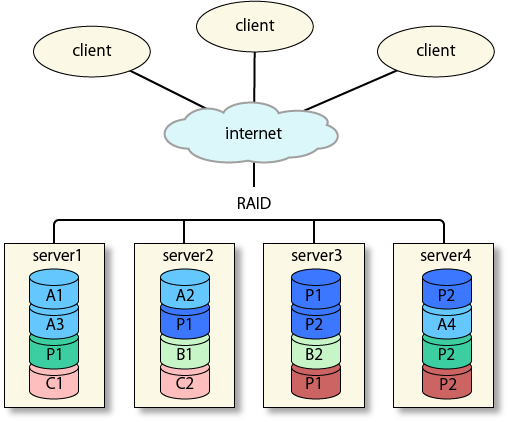
\includegraphics[clip,width=10.0cm]{images/image1.png}
		\caption{Visão geral do sistema}
		\label{fig:vis_sis}
	\end{center}
\end{figure}

Em um sistema de arquivos local, normalmente o metadado e o conteúdo de um arquivo são armazenados na mesma unidade de armazenamento. No caso de um SAD, como um arquivo pode ser armazenados distribuidamente entre servidores diferentes, os metadados são espalhados por vários servidores, tendo assim, a necessidade de fazer a busca para acessar em um determinado metadado. Obviamente essa busca consome recursos operacionais, relativamente alta por tratar de uma transmissão na rede.   \\

\begin{figure}[htb]
	\begin{center}
		
		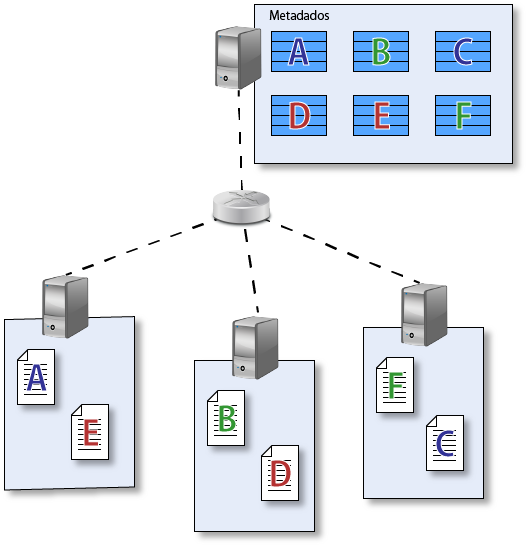
\includegraphics[clip,width=10.0cm]{images/image7.png}
		\caption{\textit{Name node} e \textit{data node}}
		\label{fig:namenode}
	\end{center}
\end{figure}

\subsection{Serviço de Metadados}
Grupo de servidores que fazem o gerenciamento dos dados.\\

Em nosso sistema utilizamos o conceito de blocos, onde um bloco é um conjunto de dados de um dado arquivo ou os dados de paridade de um determinado arquivo. O tamanho do bloco é determinado levando em consideração a quantidade de servidores de armazenamento ativos, ou seja, se houverem quatro servidores ativo, então o arquivo (independente de seu tamanho) será dividido em quatro blocos de tamanhos idênticos, caso seja necessário, o ultimo bloco será preenchido com bits '0' até que o bloco alcance o tamanho previamente fixado.
\\ 

O Serviço de metadados, também conhecido por \textit{name node}, é o conjunto de servidores que gerencia as informações dos arquivos armazenados, utilizando-se dos metadados. Em nosso sistema a data de criação, data da ultima modificação, data do ultimo acesso, tamanho, identificador do bloco de dados e nome do servidor são considerados metadados. 
\\

É da responsabilidade do sistema de metadados gerenciar a comunicação entre cliente e servidores de armazenamento (ou  \textit{data nodes}), utilizando-se das informações que indicam  estado atual do sistema e qual o tipo de RAID está sendo utilizado (apenas um tipo de RAID pode ser utilizado por operação) o \textit{name node} deve decidir em quantos blocos de tamanho idêntico o arquivo deve ser dividido e em quais servidores de armazenamento cada bloco deve ser armazenado.
\\ 

Nosso sistema está preparado para tratar os seguintes tipos de RAID, os quais foram explorados com maior profundidade no capítulo 4.
\\

\begin{itemize}
	\item RAID 0 - fracionamento simples;
	\item RAID 1 - espelhamento;
	\item RAID 5 - fracionamento com paridade espalhada entre os discos do vetor.
\end{itemize}

O Serviço de metadados mantém na sua memória local a árvore de diretórios, o que indica localização lógica dos arquivos. Quando recebe uma solicitação de cliente por um arquivo, pesquisa a sua árvore de diretórios para identificar qual diretório que este arquivo se encontra. Como resultado da pesquisa obtém o metadado do arquivo referente, conseguindo descobrir a sua localização física, a lista dos todos os \textit{data nodes} que possuem as partes do arquivo.
\\

Por sua propriedade como um interface entre clientes e \textit{data nodes}, a ocorrência de alguma falha na operação ou indisponibilidade causada pela queda do servidor tem  enorme influencia na execução do sistema, podendo até resultar em parada total do sistema. Assim, é muito importante elaborar uma esquema para manter o \textit{name node} protegidos contra falhas ou queda total. Em nosso sistema usaremos a biblioteca BFT-SMaRt, que fornece tolerância a falha no serviço através de replicação por máquina de estado. \\

\subsection{Serviço de Armazenamento}
Grupo de servidores responsáveis pelo armazenamento físico dos dados gerenciados pelo sistema de metadados. Também conhecido como \textit{data nodes}.\\

Em nosso sistema, o serviço de armazenamento não possui a necessidade de saber qual tipo de RAID está sendo executado, a responsabilidade de manter o RAID consistente é toda do serviço de metadados. Desta forma, o sistema de armazenamento apenas se conecta a uma porta e fica aguardando algum cliente se conectar a sua respectiva porta. Quando algum cliente conecta-se na porta do servidor, é realizado um \textit{handshake} preliminar, logo em seguida o cliente inicia a transferência dos dados que devem ser guardados pelo sistema de armazenamento. Ao fim da transferência o cliente fecha a conexão, enquanto o sistema de armazenamento indexa o arquivo recebido utilizando as informações adicionais que o serviço de metadados anexou ao arquivo. Com tais informações é possível saber o identificador tanto do arquivo quanto do cliente que o enviou. Tais dados adicionais são necessários para garantir que apenas o usuário dono dos dados enviados tenha acesso a eles, além de possibilitar identificar quais dados o cliente deseja receber de forma simples e eficiente.  
\\

\subsection{Cliente}
O programa cliente executado no computador do usuário final de nosso sistema. 
\\

Para cada operação que deseje realizar, o programa cliente (doravante Cliente) deve primeiramente comunicar-se com o serviço de metadados, o qual ou irá realizar a operação (no caso de operações envolvendo diretórios) ou informar com quais servidores de armazenamento o cliente deve se comunicar e quais blocos devem ser enviados para cada servidor (no caso de operações envolvendo arquivos). Entretanto, é função do Cliente informar qual tipo de RAID ele deseja utilizar.
\\

Após a comunicação inicial com o serviço de metadados, caso o cliente solicite pelo \textit{upload} ele deve iniciar a comunicação com os servidores de dados informados pelo serviço de metadado. Caso o cliente tenha decidido utilizar o RAID 5, é ele quem fica responsável por calcular a paridade do arquivo, isto deve-se ao fato de que apenas o cliente conhece o arquivo. O procedimento para o calculo da paridade é exemplificado na figura~\ref{fig:img6}. Outra atribuição do cliente é a partição do arquivo em blocos de iguais tamanhos, cada bloco será enviado para um dos servidores de dados informado pelo metadado, ou seja, o arquivo deve ser fragmentado de tal forma que cada servidor receba um bloco de dados, frisando que no caso do RAID 5 um dos blocos deve conter apenas informações de paridade previamente calculado pelo cliente. 
\\

\begin{figure}[htb]
	\begin{center}
		
		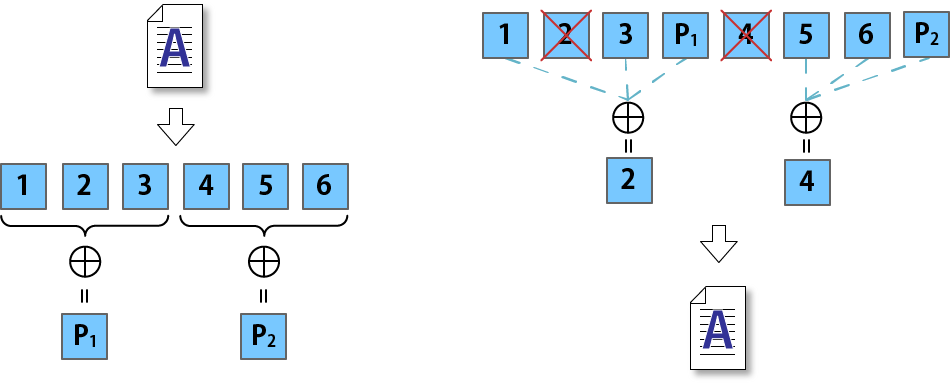
\includegraphics[clip,width=15.0cm]{images/image6.png}
		\caption{Geração de paridade}
		\label{fig:img6}
	\end{center}
\end{figure}

Caso a operação desejada pelo usuário final seja a de \textit{download} de algum de seus arquivos, o cliente deve coletar as informações de quais servidores possuem os blocos do arquivo almejado e quais as informações de identificação de cada bloco através do servidor de metadado. Com posse de tais informações, o cliente deve iniciar a comunicação com cada um dos servidores de dados apresentando a identificação de qual bloco cada servidor de dados deve enviar. Quando todos os servidores acabarem seus envios, o cliente deve usar os dados em sua posse para unir todos os blocos e recriar o arquivo desejado pelo usuário. Obviamente, esta descrição genérica da operação vai sofrer leves alterações dependendo de qual opção de RAID o cliente esteja utilizando. Para a opção de RAID 5, é possível que um dos blocos recebidos pelo cliente seja um bloco de paridade, para esse caso, o cliente deve utilizar as informações dos outros blocos para determinar qual é o bloco de dados faltante e utilizar a paridade para recuperar tal bloco. A Figura~\ref{fig:img2} mostra um esquema simplificado da operação de recuperar um arquivo realizado pelo lado do cliente.
\\

\begin{figure}[htb]
	\begin{center}
		
		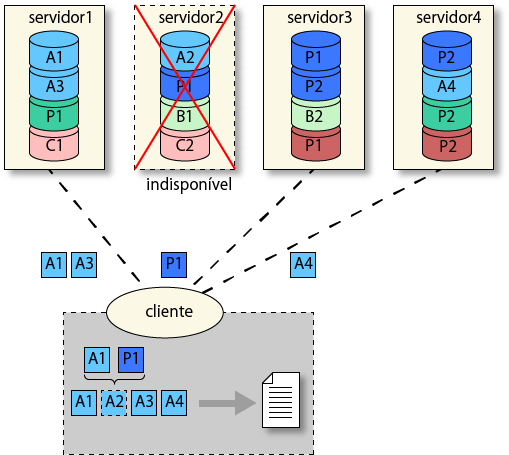
\includegraphics[clip,width=10.0cm]{images/image2.png}
		\caption{Recuperando um arquivo de uma falha}
		\label{fig:img2}
	\end{center}
\end{figure}

\section{Operações no Sistema de Arquivos Distribuídos}

Nesta seção serão apresentadas as operações básicas que o nosso SAD executa. Tais operações podem ser divididas em dois grupos dependendo das entidades envolvidas. O primeiro deles é entre cliente e servidor, composta por operações envolvendo solicitações de ações do cliente para o servidor. O segundo tipo é as operações que ocorrem entre servidores, voltadas para o gerenciamento do serviço sendo que este tipo de operações deve ocorrer de forma transparente para o cliente.
\\

\subsection{Cliente-Servidor}

É um conjunto de operações semelhantes as que são implementadas em um sistema de arquivos local, aquele que é integrado na maioria dos sistemas operacionais centralizados. Composto pelas operações sobre arquivo, pastas e suas execuções ocorrerem entre cliente e \textit{name node} ou \textit{data node}.

\subsubsection{Criar arquivo}

Operação realizada inicialmente entre o cliente e o servidor do tipo \textit{name node}. Nesse primeiro momento o cliente informa ao \textit{name node} que deseja criar um novo arquivo e em qual diretório ele deve ser criado, além de enviar os metadados do arquivo que pretende enviar. Com posse dessas informações e de qual RAID o cliente está operando, o servidor de metadados processa e transmite para o cliente para quais \textit{data node} os blocos do arquivo devem ser enviados e qual a identificação de cada bloco. O processamento de tais informações é diretamente influenciado pelo estado atual do sistema, o \textit{name node} leva em consideração a disponibilidade de cada \textit{data node} e o quanto de espaço livre em disco cada um possui.
\\

A segunda parte da operação é realizada entre o cliente e os servidores do tipo \textit{data node}. Após a comunicação com o servidor de metadados, o cliente sabe para quantos \textit{data nodes} o seu arquivo será enviado, desta forma, o cliente fragmenta o arquivo de forma que cada \textit{data nodes} irá receber um bloco de tamanho uniforme. Caso o sistema esteja usando o RAID 5, o cliente ainda deve calcular o bloco de paridade do arquivo e enviar para um dos \textit{data nodes}.
\\

\subsubsection{Criar diretório}

Operação realizada exclusivamente entre o cliente e o servidor \textit{name node}. Nessa operação o cliente informa ao \textit{name node} que deseja criar um diretório, passando como metadados apenas o nome do novo diretório e o nome de seu diretório pai. Com tais informações, o servidor de metadados primeiramente verifica se já existe um diretório com o mesmo nome no diretório pai, em caso negativo ele atualiza a arvore de diretório do cliente. No caso de já existir um diretório com mesmo nome, o cliente é informado e o novo diretório não é criado.
\\

\subsubsection{Abrir arquivos}

Operação realizada inicialmente entre o cliente e o servidor do tipo \textit{name node}. Nesse primeiro momento o cliente informa ao \textit{name node} que deseja abrir um arquivo, para tal, o cliente deve fornecer o nome do arquivo e o nome do diretório onde ele está. A primeira ação do servidor de metadados é verificar se o arquivo de fato existe no diretório informado, em caso positivo ele deve verificar se o cliente possui acesso ao arquivo. No caso do cliente possuir acesso, o \textit{name node} verifica em quantos blocos o arquivo foi dividido e em quais \textit{data nodes} cada bloco foi armazenado, após coletar tais informações, o servidor de metadados informa ao cliente quais servidores de dados ele, o cliente, deve se comunicar e o identificador de cada bloco. Para o caso de o arquivo não existir no diretório informado ou do cliente não possuir acesso para tal arquivo, o servidor de metadados deve envia ruma mensagem de erro informando a indisponibilidade do arquivo solicitado. 
\\

A segunda parte da operação é realizada entre o cliente e os servidores do tipo \textit{data node}. Após a comunicação com o servidor de metadados, o cliente sabe em quais \textit{data nodes} os blocos de seu arquivo estão armazenados. Desta forma, o cliente inicia a comunicação com cada \textit{data node} informado. A comunicação procede da seguinte forma, o cliente informa o identificador do bloco que deseja receber, enquanto que o \textit{data node} apenas verifica a existência do bloco informado. Em caso positivo, o bloco é enviado para o solicitante e em caso negativo, uma mensagem de erro alertando sobre a inexistência do bloco informado. Repare que o \textit{data node} não realiza nenhuma operação de controle de acesso sobre o bloco.
\\

A terceira parte da operação é realizada exclusivamente pelo cliente. Nesta ultima parte, o cliente é responsável por unir todos os blocos recebidos e recriar o arquivo almejado.  Vale ressaltar que essa operação sofre variações dependo do RAID sendo utilizado. Para o caso do RAID 5, um dos blocos recebido pelo cliente pode ser um bloco de paridade, nesse caso, antes de recriar o arquivo o cliente deve utilizar as informações de paridade contidas em tal bloco para recuperar o bloco faltante.
\\

\subsubsection{Abrir diretório}

Operação realizada exclusivamente entre o cliente e o servidor \textit{name node}. Nessa operação o cliente informa ao \textit{name node} que deseja abrir um diretório, passando como metadados apenas o nome do novo diretório almejado e do diretório atual. A primeira ação do servidor de metadados é verificar a existência do diretório solicitado, em caso positivo, o servidor também checa se o cliente possui permissão de acesso e se o diretório está livre. Caso todas as validações sejam positivas, o servidor muda o diretório atual do cliente para o diretório solicitado. Caso algum problema seja detectado, uma mensagem de erro é disparada para o cliente e o seu diretório atual não é alterado.
\\


\subsubsection{Deletar arquivos}

Operação realizada primeiramente entre o cliente e o servidor \textit{name node}. Nessa operação o cliente informa ao \textit{name node} que deseja deletar um arquivo, em seguida deve informar o nome do diretório onde o arquivo está armazenado e o nome do arquivo. Com tais informações, o servidor de metadados percorre a árvore de diretórios em busca do diretório requisitado, caso seja encontrado, inicia uma pesquisa pelo arquivo informado, se o arquivo for encontrado, o \textit{name node} verifica se o cliente possui permissão de acesso ao arquivo e se ele não está em estado de bloqueio, em caso positivo o arquivo é deletado da lista do metadado e a árvore de diretório do cliente atualizada. Antes de finalizar a conexão, o serviço de metadados informa ao cliente os dados sobre os blocos que compõe o arquivo.
\\

A segunda parte da operação é realizada entre o cliente e os \textit{data nodes}, onde o cliente inicia uma conexão com cada servidor de dados onde um bloco do seu arquivo está armazenado e os informam que o referido bloco deve ser deletado.
\\

\subsubsection{Deletar diretório}

Operação realizada exclusivamente entre o cliente e o servidor \textit{name node}. Nessa operação o cliente informa ao \textit{name node} que deseja deletar um diretório, passando apenas o nome do diretório almejado. A primeira ação do servidor de metadados é verificar a existência do diretório solicitado, em caso positivo, o servidor também checa se o cliente possui permissão de acesso e se o diretório está livre. Caso todas as validações sejam positivas, o servidor deleta o diretório, além de todos os arquivos contidos nele. Em seguida o servidor de metadados atualiza a árvore de diretórios do cliente.
\\

\subsubsection{Fechar um arquivo aberto}

Operação realizada exclusivamente entre o cliente e o servidor \textit{name node}. Nessa operação o cliente informa ao \textit{name node} que deseja fechar um arquivo. Primeiramente o servidor de metadados verifica se existe algum arquivo aberto pelo cliente, caso exista, é apresentado ao cliente a lista de arquivos abertos para que ele selecione qual ele deseja fechar. Sabendo qual arquivo deve ser fechado, o \textit{name node} libera o acesso ao \textit{lock} do arquivo, desta forma fechando o arquivo. Para o caso de o cliente não ter nenhum arquivo aberto é soltado uma mensagem de erro explicativa para o usuário.
\\

\subsubsection{Fechar diretório}

Operação realizada exclusivamente entre o cliente e o servidor \textit{name node}. Nessa operação o cliente informa ao \textit{name node} que deseja fechar o diretório. Primeiramente o servidor de metadados verifica se o diretório atual é o diretório raiz, caso seja, o cliente é informado que não pode fechar o diretório raiz. Caso não seja o raiz, o diretório atual é atualizado para o diretório pai do antigo diretório atual.
\\

\subsubsection{Editar um arquivo}

Operação realizada inicialmente entre o cliente e o servidor do tipo \textit{name node}. Nesse primeiro momento o cliente informa ao \textit{name node} que deseja editar um arquivo, para tal, o cliente deve fornecer o nome do arquivo. Em posse do nome do arquivo, o servidor de metadado verifica sua existência no diretório corrente, em caso positivo ainda é preciso confirmar se o arquivo já está aberto. Verificado que o arquivo não encontra-se aberto, as informações sobre o arquivo são passados para o cliente. Com tais informações, a operação que o cliente realiza é a exclusão do antigo arquivo seguida da criação do novo (ou seja, a atualização do antigo arquivo). Tais operações são realizadas como descrito previamente, entretanto, com a diferença que o usuário não precisa informar o nome do arquivo pois ele é criado com o mesmo nome do antigo.
\\

\subsubsection{Renomear um arquivo}
Operação realizada entre o cliente e o servidor \textit{name node}. Nessa operação o cliente informa ao \textit{name node} que deseja renomear um arquivo, além de fornecer o nome do arquivo que deve ser renomeado ele também deve informar o novo nome. Primeiramente o servidor de metadados procura pelo arquivo informado no diretório corrente, caso o arquivo seja encontrado ainda é necessário que o \textit{name node} verifique se o cliente possui permissão de acesso ao arquivo e se o mesmo não está aberto, caso o arquivo esteja fechado e o cliente tenha permissão de acesso, o arquivo é, enfim, renomeado com o novo nome.
\\

\subsubsection{Renomear Diretório}

Operação realizada exclusivamente entre o cliente e o servidor \textit{name node}. Nessa operação o cliente informa ao \textit{name node} que deseja renomear o diretório, além de fornecer o nome do diretório que deve ser renomeado e o seu novo nome. Primeiramente o servidor de metadados percorre a árvore de diretórios em busca do nome fornecido, caso seja encontrado o diretório é renomeado com o novo nome fornecido pelo cliente e seu metadado referente a sua ultima modificação é atualizado.
\\

%	\subsection{Servidor-Servidor}
%	São operações realizadas entre os \textit{name nodes} e os \textit{data nodes}, com função de gerenciamento do Sistema de Arquivos Distribuídos.

%	\subsubsection{Receber arquivo criado}

%	Na operação de criar arquivo, o \textit{name node} define quais \textit{data nodes} vão ser utilizados para armazenar os fragmentos de arquivo a ser criado, calculando a melhor forma para distribuir igualmente a carga entre os \textit{data nodes}. Dessa forma, além de informar ao cliente quais são os servidores para os quais deve enviar os dados, também deve avisar aos \textit{data nodes} que um cliente irá iniciar uma transferência de dados.

%	\subsubsection{Apagar arquivo deletado}

%	Além das ações entre o \textit{name node} e o cliente explanadas na subseção anterior, para efetivamente deletar um arquivo, o \textit{name node} também....

%	Deleta os dados pertencentes ao arquivo solicitado para exclusão.

%	\subsubsection{Transferir dados entre servidores}

%	Transferência de arquivos entre \textit{data nodes}.


\section{Implementação}
Nesta seção serão apresentados os detalhes sobre a implementação do nosso sistema, incluindo informações sobre a programação e algoritmos utilizados. Todo o \textit{software} foi desenvolvido na linguagem \textit{Java} com auxilio de várias bibliotecas padrões e do \textit{BFT-SMaRt}, o qual foi apresentado com mais detalhes no capítulo 3. 
\\

\subsection{Executando o Sistema}
O código-fonte de todo o projeto pode ser encontrado no repositório do \textit{GitHub}, no seguinte endereço você pode ter acesso aos arquivos \href{https://github.com/diogoAF/tccRAID}{https://github.com/diogoAF/tccRAID}. Vale ressaltar que todas as bibliotecas necessárias, incluindo o  \textit{BFT-SMaRt}, já estão incluídas no projeto. Para a execução do sistema é necessário ao menos oito máquinas remotas, sendo três máquinas para o serviço de metadado, quatro para o serviço de armazenamento (caso vá utilizar o RAID 0 ou 1, devido a sua natureza, é possível ser utilizado com apenas duas máquinas), e ao menos uma máquina rodando o Cliente.
\\

O primeiro passo é criar o arquivo \textbf{host.config} dentro de um diretório chamado \textbf{config}. Localizado no diretório \textbf{bin} existe um modelo de construção deste arquivo. Ele é necessário pois é utilizado pelo \textit{BFT-SMaRt} para determinar o IP e porta de cada réplica. Ao final do arquivo deve-se inserir uma nova linha contendo o ID do servidor, endereço IP e porta pela qual ele vai escutar. Por exemplo, 7001 10.1.1.9 11100.
\\

O segundo passo é inicializar o serviço de metadado, para tal deve-se chamar a classe \textit{server.meta.ServerConsole}, a qual deve receber quatro parâmetros os quais serão listado a seguir. 
 
\begin{itemize}
	\item O identificador único da replica;
	\item O tipo do RAID que será utilizado;
	\item O número de servidores de armazenamento;
	\item "true" caso deseje rodar a versão \textit{verbose} do metadado.
\end{itemize}

Porém, antes de executar o comando de inicialização, recomenda-se criar um \textit{script} que inicialize o \textit{BFT-SMaRt} e as outras bibliotecas, para tal, basta seguir o formato apresentado a logo abaixo, para conveniência, doravante vamos supor que o \textit{script} foi criado e chama-se \textit{scriptBftSmart.sh}.

\begin{lstlisting}
java -cp .:lib/BFT-SMaRt.jar:lib/slf4j-api-1.5.8.jar:lib/slf4j-jdk14-1.5.8.jar:lib/netty-3.1.1.GA.jar:lib/commons-codec-1.5.jar $1 $2 $3 $4 $5 $6 $7 $8 $9
\end{lstlisting}

Com o \textit{script} criado, basta rodar o seguinte comando (cada um em cada máquina), repare que cada máquina irá receber um identificador único, entretanto, o restante dos parâmetros são inalterados. Repare que é na inicialização do serviço de metadados que o tipo de RAID é determinado e ele não pode ser alterado em tempo de execução. Neste exemplo o serviço está sendo iniciado para tratar o RAID 0 com quatro servidores de armazenamento e com \textit{verbose.}
\\

\begin{lstlisting}
sh scriptBftSmart.sh server.meta.ServerConsole 0 0 4 true
sh scriptBftSmart.sh server.meta.ServerConsole 1 0 4 true
sh scriptBftSmart.sh server.meta.ServerConsole 2 0 4 true
\end{lstlisting}

Com os servidores de metadado devidamente inicializados, deve iniciar o serviço de armazenamento. A classe que deve ser invocada é a \textit{server.data.ServerConsole}, a qual deve receber dois parâmetros, os quais serão listado a seguir. 

\begin{itemize}
	\item O identificador único da replica;
	\item "true" caso deseje rodar a versão \textit{verbose} do servidor de armazenamento.
\end{itemize}

No exemplo a seguir, o serviço será instanciado com quatro servidores com o \textit{verbose} ativado.

\begin{lstlisting}
sh scriptBftSmart.sh server.data.ServerConsole 1001 true
sh scriptBftSmart.sh server.data.ServerConsole 1002 true
sh scriptBftSmart.sh server.data.ServerConsole 1003 true
sh scriptBftSmart.sh server.data.ServerConsole 1004 true
\end{lstlisting}

Nesse ponto o serviço de metadados já deve ter estabelecido conexão com os servidores de dados. Desta forma, só o que falta é ativar o cliente. Para tal, é possível ativa-lo de dois modos, o real e o de testes. No modo real será apresentado uma interface de \textit{prompt} onde o usuário poderá interagir informando qual operação ele deseje que o sistema execute. Enquanto que no modo de teste é passado na linha de comando qual operação deve ser executada (r para leitura ou w para escrita), o tamanho do arquivo de teste (1,100,1000 ou 10000 todos em kilobytes), a quantidade de \textit{threads} que serão instanciadas e a quantidade de operações. Os arquivos que são utilizados no modo de teste também podem ser encontrados na pasta \textbf{bin }.
\\

Para executar um cliente em modo real, é necessário chamar a classe \textit{client.ClientConsole}, a qual recebe apenas o identificador do cliente como parâmetro. No exemplo a seguir, é inicializado um cliente de id 7001.
\\

\begin{lstlisting}
sh scriptBftSmart.sh client.ClientConsole 7001
\end{lstlisting}

No caso do cliente em modo de teste, deve-se chamar a classe \textit{client.ClientTest}, a qual teve seus parâmetros de entrada explicados no paragrafo anterior. Desta forma, no exemplo a seguir o cliente de teste vai instanciar 10 \textit{threads} onde cada uma irá executar 500 operações de escrita do arquivo de 1kb.

\begin{lstlisting}
sh scriptBftSmart.sh client.ClientTest 7001 w 1 10 500
\end{lstlisting}
	
\subsection{Serviço de Metadados}
Nesta seção a implementação do Serviço de Metadados será detalhada. O serviço supracitado foi desenvolvido em quatro classes, as quais são listadas a seguir.
\\

\begin{itemize}
	\item RaidType;
	\item ServerConsole;
	\item ServerList;
	\item ServerMeta.
\end{itemize}

A classe \textbf{ServerConsole} serve apenas como uma interface de inicialização do serviço de metadados, no qual o \textit{ServerConsole} verifica os parâmetros de inicialização, caso tenha algo errado é apresentado uma mensagem de erro e o programa finalizado. Em contra partida, se tudo estiver correto com os parâmetros, a classe \textit{ServerMeta} é instanciada.
\\

A classe \textbf{RaidType} é apenas uma enumeração contendo os tipos de RAID suportados pelo sistema, ou seja, 0, 1 e 5.
\\

\textbf{ServerList } é a classe responsável pelas operações relacionadas ao \textit{ArrayList} contendo as informações referentes aos servidores de armazenamento cujo o serviço de metadado matem conexão.
\\

Diferente das classes supracitadas, \textbf{ServerMeta} é a classe principal do serviço de metadados. Ela é responsável por inicializar, gerenciar todo o serviço, além de executar as operações solicitadas pelos clientes. As operações disponíveis já foram apresentadas em detalhes na seção Operações no Sistema de Arquivos Distribuídos.
\\

Como mostra na parte de código abaixo, o \textit{ServerMeta} herda as características da classe \textit{DefaultSingleRecoverable}, que é contida na biblioteca \textit{BFT-SMaRt}.
Nesta classe são implementadas as funcionalidade para que a máquina que executa este código tenha papel de servidor, no contexto de \textit{BFT-SMaRt}, fazendo a replicação de serviço do sistema. 

\begin{lstlisting}[basicstyle=\ttfamily\footnotesize, frame=single]		
public class ServerMeta extends DefaultSingleRecoverable {
	
			...
		
	public ServerMeta(int id){
		new ServiceReplica(id, this, this);
		dt   = new DirectoryTree();
		list = new ServerList(); 
	}

			...
\end{lstlisting}	

O método mostrado abaixo serve para atender à requisição pela operações que a ordem da execução precisam ser considerados.
Primeiro recebe o tipo de operação para ser executado, e depois chama o método adequado para continuar com o processo.
As operações que podem ser processados em qualquer ordem são atendidas por método \textit{appExecuteUnordered}.

\begin{lstlisting}[basicstyle=\ttfamily\footnotesize, frame=single]		
public byte[] appExecuteOrdered(byte[] command, MessageContext msgCtx) {
			
			...
			
	byte[] resultBytes = null;
	
	try {
		ByteArrayInputStream in  = new ByteArrayInputStream(command);
		ObjectInputStream    ois = new ObjectInputStream(in);
		
		int reqType = ois.readInt();
		
		switch(reqType) {
			case RequestType.CREATEDIR:
			resultBytes = criateDir(ois);
			break;
			
			case RequestType.DELETEDIR:
			resultBytes = deleteDir(ois);
			break;

			...
\end{lstlisting}	

Todos os métodos desta classe possuem um fluxo de execução padronizado desta forma; recebe requisição, processa a operação e retorna o resultado. 
O método \textit{open} abaixo, que faz operação de abrir um arquivo, mostra o fluxo apresentado.

\begin{lstlisting}[basicstyle=\ttfamily\footnotesize, frame=single]		
private byte[] open(ObjectInputStream ois) throws ClassNotFoundException, IOException {
	String   currPath = (String)ois.readObject();
	String   tgtName  = (String)ois.readObject();
	long     accTime  = ois.readLong();
	
			...
	
	Directory currDir   = dt.openDirectory(currPath, accTime);
	int       result    = -1;
	long      fileSize  = 0;
	FileDFS   target    = null;
	BlockInfoList bList = null;
	
	if(currDir == null) {
		currDir = dt.getRoot();
		result  = ResultType.FAILURE;
	} else if(!currDir.existFile(tgtName)) {
		result = ResultType.FILENOTEXISTS;
	} else {
		target = currDir.getFile(tgtName);
		if( ( target.isLokedW() ) &&
			( System.currentTimeMillis()-target.getLastAccTime() ) <= 30*1000 ) 
		{
			result = ResultType.FILELOCKED;
		} else {
			target.lockR();
			bList  = target.getBlockList();
			fileSize = target.getMetadata().size();
			result = ResultType.SUCCESS;
		}
	}

	ByteArrayOutputStream out = new ByteArrayOutputStream();
	ObjectOutputStream    oos = new ObjectOutputStream(out);

	oos.writeInt(result);
	oos.writeObject(currDir.getDirEntries());
	oos.writeObject(bList);
	oos.writeLong(fileSize);
	oos.flush();
	
			...
				
	return out.toByteArray();
}
\end{lstlisting}


Além das classes supracitadas, o \textit{package} do serviço de metadados trabalha diretamente com os \textit{packages} responsáveis por gerenciar todas as estruturas de diretório do sistema, por isso tais classes serão apresentadas nesta subseção e explanadas em breve.
\\

\begin{itemize}
	\item \textbf{dt}
	\begin{itemize}
		\item DirectoryNode;
		\item DirectoryTree;
		\item LockList;
		\item LockType;
		\item Metadata.
	\end{itemize}
	\item \textbf{dt.directory}
	\begin{itemize}
		\item DirEntries;
		\item Directory.
	\end{itemize}
	\item \textbf{dt.file}
	\begin{itemize}
		\item Block;
		\item BlockInfo;
		\item BlockInfoList;
		\item FileDFS.
	\end{itemize}
\end{itemize}

As classes contidas no \textit{package dt} lidam com todas características e operações refentes aos diretórios. \textbf{LockType e LockList} são utilizadas para gerenciar o controle de acesso aos diretórios, sendo a primeira responsável por enumerar os tipos dos estados de acesso dos diretórios, enquanto a segunda gerência um \textit{ArrayList} para listar os arquivos contidos no diretório e seu controle de acesso. A classe \textbf{Metadata} contêm e manipula as informações de metadado dos arquivos. Por fim, \textbf{DirectoryNode e DirectoryTree} compõem a árvore de diretórios do serviço de metadados, a primeira referente a cada nó e a segunda sobre a árvore em si.
\\

Dentro de dt, existem dois outros \textit{packges}, sendo \textit{directory} responsável por tratar os diretórios em si. Composto por duas classes, \textit{DirEntries e Directory}, sendo o primeiro composto pelas informações das entidades armazenadas nos diretórios (outros diretórios e/ou arquivos) e um método para informar se o diretório referenciado é ou não o \textit{root}, enquanto que a segunda trata dos diretórios em si composto por vários métodos de operações sobre pastas e dois \textit{HashMaps} para armazenar as informações das pastas e arquivos contidos no diretório referenciado.
\\

Por fim, o outro \textit{packge} dentro de dt é nomeado de \textit{file}, o qual compõem as classes responsáveis por armazenar e gerenciar os dados dos arquivos armazenados pelo serviço de armazenamento. \textbf{FileDFS} é a classe principal deste \textit{packge}, contendo a referencia da instância de \textit{BlockInfoList}. \textbf{Block, BlockInfo e BlockInfoList} referentes aos blocos de dados nos quais os arquivos devem ser divididos antes de serem enviados pelo cliente ao serviço de armazenamento. Dentre as classes previamente sitadas,\textit{Block} pode ser considerada como a principal, visto que é nela onde ficam armazenados os \textit{bytes} de dados, o identificador e os metodos necessários para recuperar os dados ou quebrar um dado arquivo em blocos. Enquanto que \textit{BlockInfo} funciona como a ligação do bloco ao servidor de armazenamento par ao qual ele deve ser enviado, contendo as informações necessárias para que o cliente saiba para quem o bloco deve ser enviado. Por fim, \textit{BlockInfoList} possui os meios para gerenciar um \textit{ArrayList} dos \textit{BlockInfo} de um arquivo, além de manter o tamanho de cada bloco da lista, o número de servidores de armazenamento eo tipo de RAID em que os blocos foram criados.
\\

\subsection{Serviço de Armazenamento}
Nesta seção a implementação do Serviço de Armazenamento será detalhada. O serviço supracitado foi desenvolvido em quatro classes, as quais são listadas a seguir.
\\

\begin{itemize}
	\item MetadataModule;
	\item ServerConsole;
	\item Operation;
	\item ServerData.
\end{itemize}

A classe \textbf{ServerConsole} serve apenas como uma interface de inicialização do serviço de armazenamento, no qual o \textit{ServerConsole} verifica os parâmetros de inicialização, caso tenha algo errado é apresentado uma mensagem de erro e o programa finalizado. Em contra partida, se tudo estiver correto com os parâmetros, a classe \textit{ServerData} é instanciada.
\\

A classe \textbf{Operation} é a classe responsável por efetivamente executar as operações solicitadas ao serviço de armazenamento sobre os blocos de arquivos.
\\

O \textit{Operation} herda a classe \textit{Thread} para realizar o processamento em \textit{multithread}.
Na parte de execução mostrado abaixo faz a chamada de método adequado de acordo com tipo de operação requerida.
\begin{lstlisting}[basicstyle=\ttfamily\footnotesize, frame=single]		
public class Operation extends Thread {
	
			...
			
public void run() {
	if(verbose)
		System.out.println("Cliente conectado do IP "
		+clientSocket.getInetAddress().getHostAddress());
	
	try {
		InputStream in = clientSocket.getInputStream();
		ObjectInputStream ois = new ObjectInputStream(in);
		
		int   reqType = ois.readInt();
		Block block   = (Block)ois.readObject();
		
		switch(reqType) {
			case(RequestType.CREATE):
				create(block);
				break;
		
			case(RequestType.DELETE):
			
			...
\end{lstlisting}



\textbf{ServerData} é a classe responsável por lidar diretamente com os clientes, de modo que é ela quem sabe a porta onde o servidor deve aguardar pela conexão do cliente, a sua capacidade total de armazenamento e quanto do espaço já foi ocupado.
\\

O trecho do código mostrado a seguir é parte principal de execução da classe \textit{ServerData}.
O fluxo começa esperando cliente,  segue para criação da instancia de \textit{Operation} e dá início à instancia criada.
\begin{lstlisting}[basicstyle=\ttfamily\footnotesize, frame=single]		
while(true) {
	iterations++;
	if(verbose)
		System.out.println("Aguardando cliente...");
	try {
		Socket clientSocket = serverSocket.accept();
		
		Operation op = new Operation(clientSocket, dirName, verbose);
		op.start();
	} catch (SocketException e) {
		e.printStackTrace();
		System.exit(0);
	}
}

			...
\end{lstlisting}

A classe \textbf{MetaDataModule} realiza a comunicação com os servidores de metadados. Tal comunicação é realizada utilizando as facilidades do \textit{BFT-SMaRt}, no qual o \textit{MetaDataModule} age no papel de um cliente solicitando algum serviço do servidor de metadados.
\\

\subsection{Cliente}
Nesta seção a implementação do Cliente será detalhada. O serviço supracitado foi desenvolvido em seis classes, as quais são listadas a seguir.
\\

\begin{itemize}
	\item ClientConsole;
	\item ClientDFS;
	\item ClientServerSocket;
	\item Option;
	\item ClientTest.
\end{itemize}

Observe que a classe \textbf{ClientTest} é utilizada apenas no modo de teste, na execução normal ela é ignorada pelo sistema e não deve ser chamada. Sua utilização foi explicada no tópico anterior.

A parte de preparação é mostrado abaixo, onde são criados vários \textit{threads} da classe \textbf{ClientDFS} e colocado para executar o teste.

\begin{lstlisting}[basicstyle=\ttfamily\footnotesize, frame=single]		
long[] values = new long[numThreads];
Client[] c = new Client[numThreads];

for (int i = 0; i < numThreads; i++) {
	try {
		Thread.sleep(100);
	} catch (InterruptedException e) {
		e.printStackTrace();
	}

	System.out.println("Launching client " + (initId + i));
	c[i] = new ClientTest.Client(values, i, opsType, numberOfOps, interval);
}
	
			...
\end{lstlisting}

Agora executa o teste chamando os métodos de acordo com tipo de  operação escolhido. 
Ao terminar a executar todas as operações, apenas a instancia de \textbf{ClientDFS} que possui número de ID igual a ID inicial imprime o resultado e termina o teste.

\begin{lstlisting}[basicstyle=\ttfamily\footnotesize, frame=single]
for (int i = 0; i < numberOfOps; i++, req++) {
	System.out.print("Sending req " + req + "...");
	
	try {
		switch(opsType) {
			case(READ):
				last_send_instant = System.nanoTime();
				cdfs.open("test_"+id+"_"+i);
				st.store(System.nanoTime() - last_send_instant);
				break;
			
			case(WRITE):
				last_send_instant = System.nanoTime();
				cdfs.create("test", "test_"+id+"_"+i);
				st.store(System.nanoTime() - last_send_instant);
				break;
			
			...
			
	if (id == initId) {
		System.out.println(this.id + " // Average time for " + numberOfOps + " executions (-10%) = " + st.getAverage(true) / 1000 + " us ");
		
			...
			
	}	
		
			...
\end{lstlisting}
 


A classe \textbf{ClientConsole} serve apenas como uma interface entre o usuário e o \textit{software}, no qual o \textit{ClientConsole} apresenta um menu baseado em linha de comando, no qual o usuário informa qual operação deseja executar, o \textit{ClientConsole} valida os dados fornecidos e avisa o módulo responsável por executar a operação desejada.
\\

O código abaixo mostra o método para executar a operação de criação de arquivo.
Basicamente todos os métodos que executa a operação possuem esta forma; interação com usuário, chamada de método do \textit{ClientDFS} e processamento de resultado.
\begin{lstlisting}[basicstyle=\ttfamily\footnotesize, frame=single]
private void create(Console con) throws ClassNotFoundException, IOException  {
	System.out.println();
	System.out.println("Criar arquivo");
	String srcName  = con.readLine("Nome ou local do arquivo:\n>");
	
	if(srcName.isEmpty())
		return;
	
	int result = c.create(srcName, null);
	
	if(result == ResultType.SUCCESS)
		System.out.println("Arquivo criado");
	else
		reportError(result);
}
\end{lstlisting}

A classe \textbf{Option} é apenas uma enumeração contendo os tipos de operações suportados pelo sistema, as quais foram apresentadas e discutidas previamente nesse trabalho.
\\

\textbf{ClientServerSocket} possibilita e gerencia as conexões \textit{Socket} realizadas entre o cliente e servidor, tal conexão são necessárias para a correta execução de operações entre o cliente e os servidores de armazenamento. As conexões entre o cliente e servidor de metadados ocorrem graças as facilidades do \textit{BFT-SMaRt}.
\\

O método \textit{open} mostrado abaixo serve para receber o bloco de arquivo, enviado por servidor de armazenamento.
Primeiramente envia o tipo de requisição junto ao informação sobre bloco de arquivo desejado e logo a seguir espera o envio de dado pelo servidor.
Para tolerar a falha da rede externa , quando detecta exceção de conexão espera por 10 segundos e inicia o processo, fazendo três tentativas.

\begin{lstlisting}[basicstyle=\ttfamily\footnotesize, frame=single]	
public byte[] open(Block block) throws ConnectException  {
	int triedCount = 0;
	
	while(true) {
		try {
			clientSocket = new Socket(blockInfo.getHostName(), blockInfo.getPort());
			System.out.println("O cliente se conectou ao servidor na porta " 
			+ blockInfo.getPort());
			
			ByteArrayOutputStream bos = new ByteArrayOutputStream();
			ObjectOutputStream    oos = new ObjectOutputStream(bos);
			
			oos.writeInt(RequestType.OPEN);
			oos.writeObject(block);
			oos.flush();
			
			OutputStream out = clientSocket.getOutputStream();
			
			out.write(bos.toByteArray());
		
			InputStream         is = clientSocket.getInputStream();
			BufferedInputStream in = new BufferedInputStream(is);
			
			while(is.available() == 0);
			
			byte[] buffer = new byte[BUFFER_SIZE];
			int length = in.read(buffer);
			System.out.println(length);
		
			return Arrays.copyOfRange(buffer, 0, length);
		} catch(ConnectException | UnknownHostException e) {
			try {
				Thread.sleep(10*1000);
			} catch (InterruptedException e1) {
				e1.printStackTrace();
				System.exit(-1);
			}
			
			triedCount++;
			if(triedCount>3) {
				System.out.println("O cliente nao conseguiu conectar no servidor");
				throw new ConnectException();
			}
		} catch (IOException e) {
			...
		}
	}
}
\end{lstlisting}

O método \textit{send} foi implementado como privada para ser chamado pelo outros métodos públicos, o \textit{create} e o \textit{delete}, que servem para fazer, respectivamente, o envido do bloco de arquivo e a requisição de deletar um bloco para servidor.
Utiliza a mesma esquema de tolerar a falha da rede externa que foi apresentado no método acima.

\begin{lstlisting}[basicstyle=\ttfamily\footnotesize, frame=single]	

public void create(Block block) throws ConnectException  {
	send(RequestType.CREATE, block);
}

public void delete(Block block) throws ConnectException  {
	send(RequestType.DELETE, block);
}

			...

private void send(int ReqType, Block block) throws ConnectException  {
	int triedCount = 0;
	
	while(true) {
		try {
			clientSocket = new Socket(blockInfo.getHostName(), blockInfo.getPort());
			System.out.println("O cliente se conectou ao servidor na porta " 
			+ blockInfo.getPort());
			
			ByteArrayOutputStream bos = new ByteArrayOutputStream();
			ObjectOutputStream    oos = new ObjectOutputStream(bos);
			
			oos.writeInt(ReqType);
			oos.writeObject(block);
			oos.flush();
			
			OutputStream out = clientSocket.getOutputStream();
			
			out.write(bos.toByteArray());
			
			clientSocket.close();
			
			return;
		} catch(ConnectException | UnknownHostException e) {
		
				...
				
		}
}
\end{lstlisting}

A classe \textbf{ClientDFS} pode ser considerada como a classe principal do lado cliente do sistema, visto que é nela onde estão concentrados os métodos para realização de todas as operações listadas em \textit{Option}.
\\
Quando o método não envolve com operação sobre arquivo faz comunicação somente com servidores de metadados.
O código abaixo mostra o método que implementa a operação de criar novo diretório, em que a requisição desta operação é enviado para servidores usando \textit{BFT-SMaRt}, através de do método \textit{invokeOrdered}.
O \textit{invokeOrdered} é chamado para requisitar as operações que a ordem de execução precisa ser considerado. Caso contrário, é chamado  \textit{invokeUnordered}.
Os métodos desta classe também possuem uma forma padrão; prepara o dado, envia para servidores, aguarda a resposta, e faz processamento restante de acordo com a resposta obtida.  
\begin{lstlisting}[basicstyle=\ttfamily\footnotesize, frame=single]	
public int criateDir(String tgtName) throws ClassNotFoundException, IOException {
	Metadata metadata = new Metadata(System.currentTimeMillis());
	
	ByteArrayOutputStream out = new ByteArrayOutputStream();
	ObjectOutputStream    oos = new ObjectOutputStream(out);
	
	oos.writeInt(RequestType.CREATEDIR);
	oos.writeObject(currPath.toString());
	oos.writeObject(tgtName);
	oos.writeObject(metadata);
	oos.writeLong(System.currentTimeMillis());
	oos.flush();
	
	byte[]  bytes   = this.proxy.invokeOrdered(out.toByteArray());
	
	ByteArrayInputStream in  = new ByteArrayInputStream(bytes);
	ObjectInputStream    ois = new ObjectInputStream(in);
	
	int result = ois.readInt();
	currDir    = (DirEntries)ois.readObject();
	
	if(result == ResultType.FAILURE) {
		currPath = currDir.getPath();
	}
	
	return result;
}
\end{lstlisting}
Quado o método envolve com a operação sobre arquivo, é necessário fazer comunicação com ambos tipos de servidores, o de metadados e o de armazenamento, como no método \textit{create} mostrado abaixo.
A comunicação com servidor de metadado possui mesma característica que foi apresentado no método acima.
No caso de comunicação com servidores de armazenamento ocorre através da classe \textit{ClientServerSocket} de forma \textit{multithread}.
Nas operações de leitura e escrita de arquivo a rotina de execução subdivide de acordo com tipo de RAID, mas o fluxo segue de forma parecida, como ocorre em alguns métodos apresentados anteriormente.
\begin{lstlisting}[basicstyle=\ttfamily\footnotesize, frame=single]	
public int create(String fileName, String tgtName) throws ClassNotFoundException, IOException  {
	int result = ResultType.FAILURE;
	try {
				...
		
		byte[]  bytes   = this.proxy.invokeOrdered(out.toByteArray());
		
				...
				
		ClientServerSocket[] css = new ClientServerSocket[nServers];
		byte [] buffer = new byte[blockSize];
		
		switch(raidType) {
			case(RaidType.RAID0):
			for(int i=0; i<nServers; i++) {
				Arrays.fill(buffer, (byte) 0);
				
				bInfo = bList.get(i);
				
				bis.read(buffer, 0, blockSize);
				
				Block block = new Block(bInfo.getID(),buffer);
				
				
				css[i] = new ClientServerSocket(bInfo, block, Option.CREATE, verbose);
				css[i].start();   
			}
			for(int i=0; i<nServers; i++) {
				css[i].join();
			}
			for(int i=0; i<nServers; i++) {
				if(css[i].failure()) {
					failure(bList.get(i));
					result = ResultType.FAILURE;
					break;
				}
			}
			break;
			
			case(RaidType.RAID1):
					
			...
			
			case(RaidType.RAID5):
			
			...
			
\end{lstlisting}